\documentclass[1p]{elsarticle_modified}
%\bibliographystyle{elsarticle-num}

%\usepackage[colorlinks]{hyperref}
%\usepackage{abbrmath_seonhwa} %\Abb, \Ascr, \Acal ,\Abf, \Afrak
\usepackage{amsfonts}
\usepackage{amssymb}
\usepackage{amsmath}
\usepackage{amsthm}
\usepackage{scalefnt}
\usepackage{amsbsy}
\usepackage{kotex}
\usepackage{caption}
\usepackage{subfig}
\usepackage{color}
\usepackage{graphicx}
\usepackage{xcolor} %% white, black, red, green, blue, cyan, magenta, yellow
\usepackage{float}
\usepackage{setspace}
\usepackage{hyperref}

\usepackage{tikz}
\usetikzlibrary{arrows}

\usepackage{multirow}
\usepackage{array} % fixed length table
\usepackage{hhline}

%%%%%%%%%%%%%%%%%%%%%
\makeatletter
\renewcommand*\env@matrix[1][\arraystretch]{%
	\edef\arraystretch{#1}%
	\hskip -\arraycolsep
	\let\@ifnextchar\new@ifnextchar
	\array{*\c@MaxMatrixCols c}}
\makeatother %https://tex.stackexchange.com/questions/14071/how-can-i-increase-the-line-spacing-in-a-matrix
%%%%%%%%%%%%%%%

\usepackage[normalem]{ulem}

\newcommand{\msout}[1]{\ifmmode\text{\sout{\ensuremath{#1}}}\else\sout{#1}\fi}
%SOURCE: \msout is \stkout macro in https://tex.stackexchange.com/questions/20609/strikeout-in-math-mode

\newcommand{\cancel}[1]{
	\ifmmode
	{\color{red}\msout{#1}}
	\else
	{\color{red}\sout{#1}}
	\fi
}

\newcommand{\add}[1]{
	{\color{blue}\uwave{#1}}
}

\newcommand{\replace}[2]{
	\ifmmode
	{\color{red}\msout{#1}}{\color{blue}\uwave{#2}}
	\else
	{\color{red}\sout{#1}}{\color{blue}\uwave{#2}}
	\fi
}

\newcommand{\Sol}{\mathcal{S}} %segment
\newcommand{\D}{D} %diagram
\newcommand{\A}{\mathcal{A}} %arc


%%%%%%%%%%%%%%%%%%%%%%%%%%%%%5 test

\def\sl{\operatorname{\textup{SL}}(2,\Cbb)}
\def\psl{\operatorname{\textup{PSL}}(2,\Cbb)}
\def\quan{\mkern 1mu \triangleright \mkern 1mu}

\theoremstyle{definition}
\newtheorem{thm}{Theorem}[section]
\newtheorem{prop}[thm]{Proposition}
\newtheorem{lem}[thm]{Lemma}
\newtheorem{ques}[thm]{Question}
\newtheorem{cor}[thm]{Corollary}
\newtheorem{defn}[thm]{Definition}
\newtheorem{exam}[thm]{Example}
\newtheorem{rmk}[thm]{Remark}
\newtheorem{alg}[thm]{Algorithm}

\newcommand{\I}{\sqrt{-1}}
\begin{document}

%\begin{frontmatter}
%
%\title{Boundary parabolic representations of knots up to 8 crossings}
%
%%% Group authors per affiliation:
%\author{Yunhi Cho} 
%\address{Department of Mathematics, University of Seoul, Seoul, Korea}
%\ead{yhcho@uos.ac.kr}
%
%
%\author{Seonhwa Kim} %\fnref{s_kim}}
%\address{Center for Geometry and Physics, Institute for Basic Science, Pohang, 37673, Korea}
%\ead{ryeona17@ibs.re.kr}
%
%\author{Hyuk Kim}
%\address{Department of Mathematical Sciences, Seoul National University, Seoul 08826, Korea}
%\ead{hyukkim@snu.ac.kr}
%
%\author{Seokbeom Yoon}
%\address{Department of Mathematical Sciences, Seoul National University, Seoul, 08826,  Korea}
%\ead{sbyoon15@snu.ac.kr}
%
%\begin{abstract}
%We find all boundary parabolic representation of knots up to 8 crossings.
%
%\end{abstract}
%\begin{keyword}
%    \MSC[2010] 57M25 
%\end{keyword}
%
%\end{frontmatter}

%\linenumbers
%\tableofcontents
%
\newcommand\colored[1]{\textcolor{white}{\rule[-0.35ex]{0.8em}{1.4ex}}\kern-0.8em\color{red} #1}%
%\newcommand\colored[1]{\textcolor{white}{ #1}\kern-2.17ex	\textcolor{white}{ #1}\kern-1.81ex	\textcolor{white}{ #1}\kern-2.15ex\color{red}#1	}

{\Large $\underline{12a_{0940}~(K12a_{0940})}$}

\setlength{\tabcolsep}{10pt}
\renewcommand{\arraystretch}{1.6}
\vspace{1cm}\begin{tabular}{m{100pt}>{\centering\arraybackslash}m{274pt}}
\multirow{5}{120pt}{
	\centering
	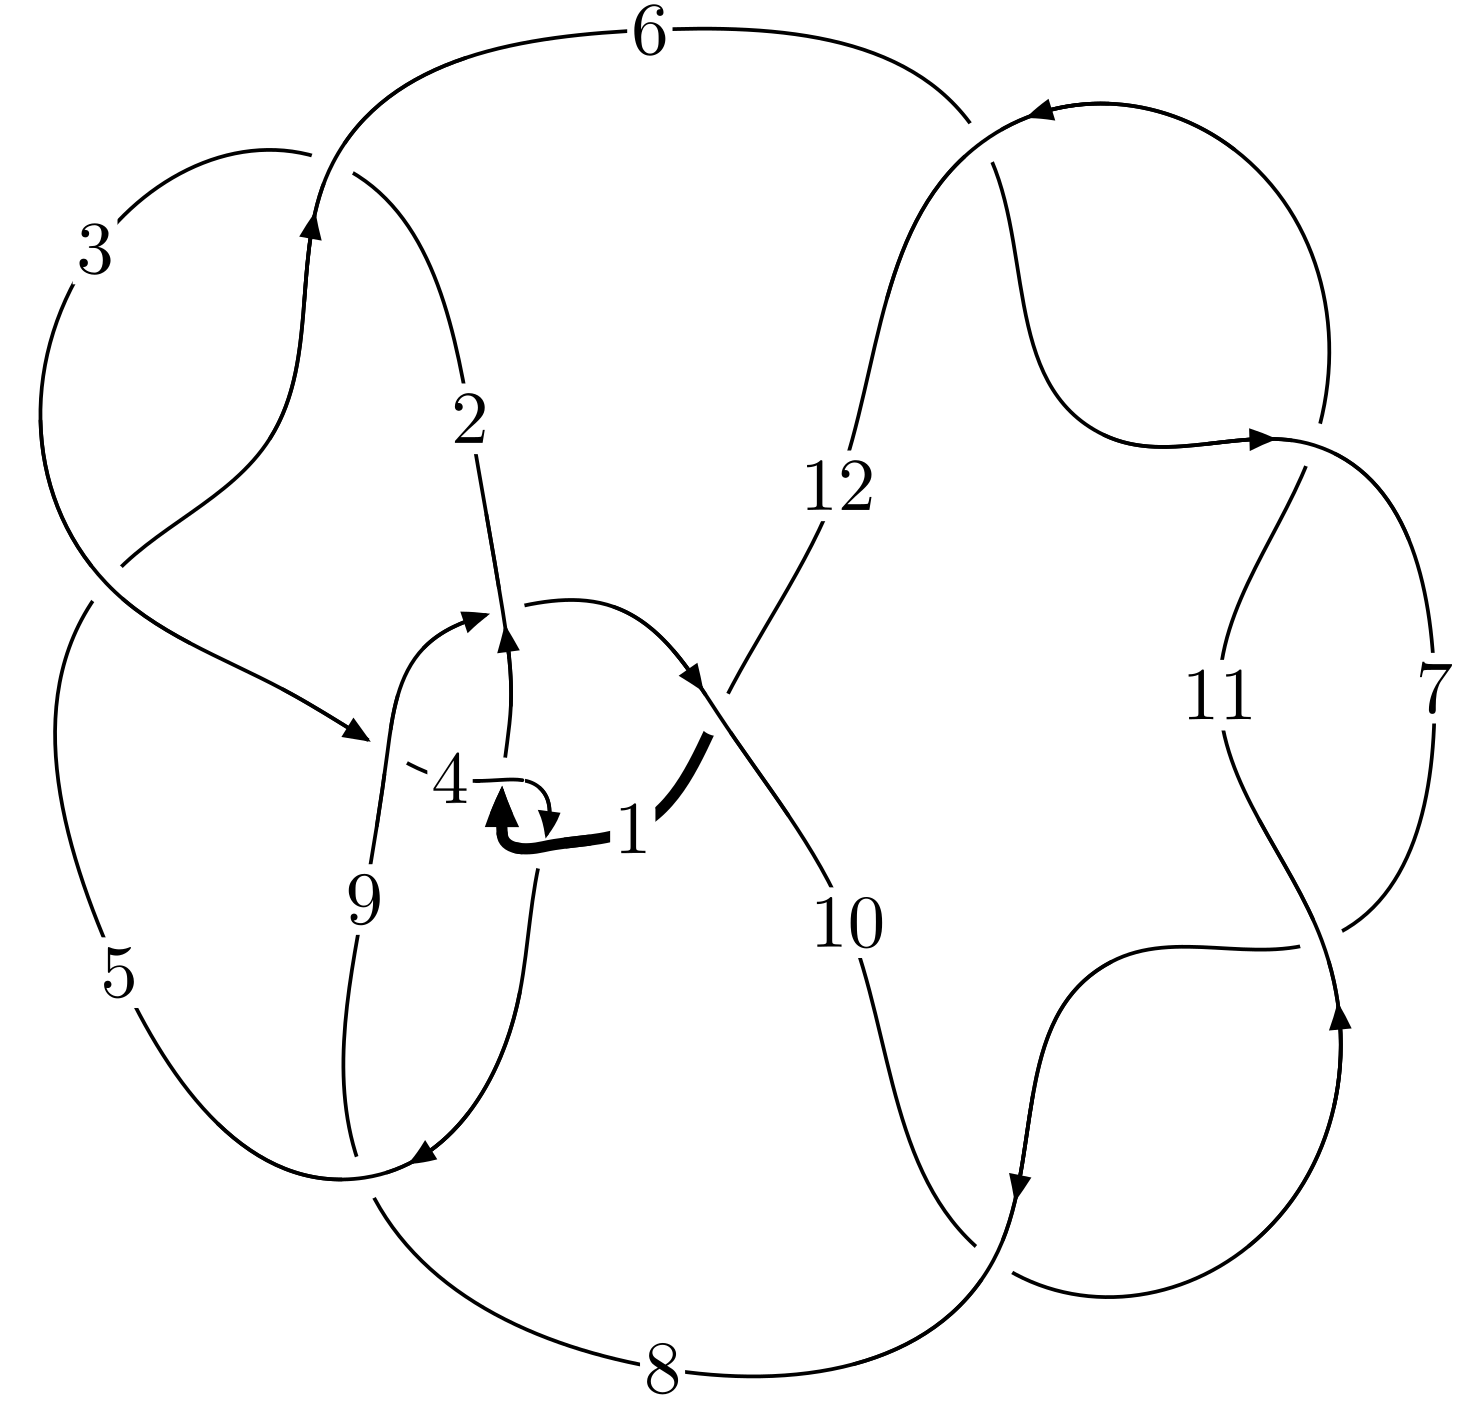
\includegraphics[width=112pt]{../../../GIT/diagram.site/Diagrams/png/1741_12a_0940.png}\\
\ \ \ A knot diagram\footnotemark}&
\allowdisplaybreaks
\textbf{Linearized knot diagam} \\
\cline{2-2}
 &
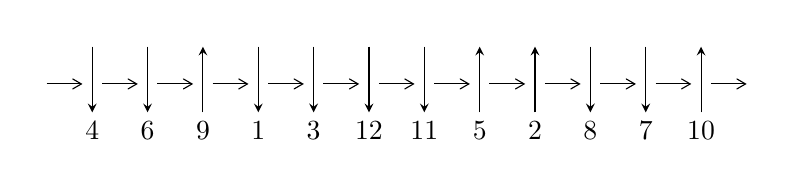
\begin{tikzpicture}[x=20pt, y=17pt]
	% nodes
	\node (C0) at (0, 0) {};
	\node (C1) at (1, 0) {};
	\node (C1U) at (1, +1) {};
	\node (C1D) at (1, -1) {4};

	\node (C2) at (2, 0) {};
	\node (C2U) at (2, +1) {};
	\node (C2D) at (2, -1) {6};

	\node (C3) at (3, 0) {};
	\node (C3U) at (3, +1) {};
	\node (C3D) at (3, -1) {9};

	\node (C4) at (4, 0) {};
	\node (C4U) at (4, +1) {};
	\node (C4D) at (4, -1) {1};

	\node (C5) at (5, 0) {};
	\node (C5U) at (5, +1) {};
	\node (C5D) at (5, -1) {3};

	\node (C6) at (6, 0) {};
	\node (C6U) at (6, +1) {};
	\node (C6D) at (6, -1) {12};

	\node (C7) at (7, 0) {};
	\node (C7U) at (7, +1) {};
	\node (C7D) at (7, -1) {11};

	\node (C8) at (8, 0) {};
	\node (C8U) at (8, +1) {};
	\node (C8D) at (8, -1) {5};

	\node (C9) at (9, 0) {};
	\node (C9U) at (9, +1) {};
	\node (C9D) at (9, -1) {2};

	\node (C10) at (10, 0) {};
	\node (C10U) at (10, +1) {};
	\node (C10D) at (10, -1) {8};

	\node (C11) at (11, 0) {};
	\node (C11U) at (11, +1) {};
	\node (C11D) at (11, -1) {7};

	\node (C12) at (12, 0) {};
	\node (C12U) at (12, +1) {};
	\node (C12D) at (12, -1) {10};
	\node (C13) at (13, 0) {};

	% arrows
	\draw[->,>={angle 60}]
	(C0) edge (C1) (C1) edge (C2) (C2) edge (C3) (C3) edge (C4) (C4) edge (C5) (C5) edge (C6) (C6) edge (C7) (C7) edge (C8) (C8) edge (C9) (C9) edge (C10) (C10) edge (C11) (C11) edge (C12) (C12) edge (C13) ;	\draw[->,>=stealth]
	(C1U) edge (C1D) (C2U) edge (C2D) (C3D) edge (C3U) (C4U) edge (C4D) (C5U) edge (C5D) (C6U) edge (C6D) (C7U) edge (C7D) (C8D) edge (C8U) (C9D) edge (C9U) (C10U) edge (C10D) (C11U) edge (C11D) (C12D) edge (C12U) ;
	\end{tikzpicture} \\
\hhline{~~} \\& 
\textbf{Solving Sequence} \\ \cline{2-2} 
 &
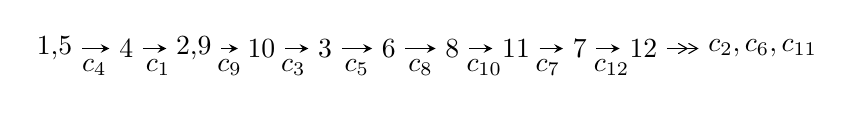
\begin{tikzpicture}[x=23pt, y=7pt]
	% node
	\node (A0) at (-1/8, 0) {1,5};
	\node (A1) at (1, 0) {4};
	\node (A2) at (33/16, 0) {2,9};
	\node (A3) at (25/8, 0) {10};
	\node (A4) at (33/8, 0) {3};
	\node (A5) at (41/8, 0) {6};
	\node (A6) at (49/8, 0) {8};
	\node (A7) at (57/8, 0) {11};
	\node (A8) at (65/8, 0) {7};
	\node (A9) at (73/8, 0) {12};
	\node (C1) at (1/2, -1) {$c_{4}$};
	\node (C2) at (3/2, -1) {$c_{1}$};
	\node (C3) at (21/8, -1) {$c_{9}$};
	\node (C4) at (29/8, -1) {$c_{3}$};
	\node (C5) at (37/8, -1) {$c_{5}$};
	\node (C6) at (45/8, -1) {$c_{8}$};
	\node (C7) at (53/8, -1) {$c_{10}$};
	\node (C8) at (61/8, -1) {$c_{7}$};
	\node (C9) at (69/8, -1) {$c_{12}$};
	\node (A10) at (11, 0) {$c_{2},c_{6},c_{11}$};

	% edge
	\draw[->,>=stealth]	
	(A0) edge (A1) (A1) edge (A2) (A2) edge (A3) (A3) edge (A4) (A4) edge (A5) (A5) edge (A6) (A6) edge (A7) (A7) edge (A8) (A8) edge (A9) ;
	\draw[->>,>={angle 60}]	
	(A9) edge (A10);
\end{tikzpicture} \\ 

\end{tabular} \\

\footnotetext{
The image of knot diagram is generated by the software ``\textbf{Draw programme}" developed by Andrew Bartholomew(\url{http://www.layer8.co.uk/maths/draw/index.htm\#Running-draw}), where we modified some parts for our purpose(\url{https://github.com/CATsTAILs/LinksPainter}).
}\phantom \\ \newline 
\centering \textbf{Ideals for irreducible components\footnotemark of $X_{\text{par}}$} 
 
\begin{align*}
I^u_{1}&=\langle 
5951 u^{31}+29371 u^{30}+\cdots+32768 b+13889,\;28929 u^{31}+106501 u^{30}+\cdots+32768 a-89345,\\
\phantom{I^u_{1}}&\phantom{= \langle  }u^{32}+4 u^{31}+\cdots+u+1\rangle \\
I^u_{2}&=\langle 
1.48022\times10^{51} u^{53}-9.91042\times10^{51} u^{52}+\cdots+4.83516\times10^{51} b+9.88707\times10^{50},\\
\phantom{I^u_{2}}&\phantom{= \langle  }4.13434\times10^{51} u^{53}-4.03971\times10^{52} u^{52}+\cdots+4.83516\times10^{51} a+1.72588\times10^{52},\;u^{54}-9 u^{53}+\cdots-2 u+1\rangle \\
I^u_{3}&=\langle 
b+a,\;16 a^4+8 a^3+4 a^2+1,\;u+1\rangle \\
\\
\end{align*}
\raggedright * 3 irreducible components of $\dim_{\mathbb{C}}=0$, with total 90 representations.\\
\footnotetext{All coefficients of polynomials are rational numbers. But the coefficients are sometimes approximated in decimal forms when there is not enough margin.}
\newpage
\renewcommand{\arraystretch}{1}
\centering \section*{I. $I^u_{1}= \langle 5951 u^{31}+29371 u^{30}+\cdots+32768 b+13889,\;28929 u^{31}+106501 u^{30}+\cdots+32768 a-89345,\;u^{32}+4 u^{31}+\cdots+u+1 \rangle$}
\flushleft \textbf{(i) Arc colorings}\\
\begin{tabular}{m{7pt} m{180pt} m{7pt} m{180pt} }
\flushright $a_{1}=$&$\begin{pmatrix}0\\u\end{pmatrix}$ \\
\flushright $a_{5}=$&$\begin{pmatrix}1\\0\end{pmatrix}$ \\
\flushright $a_{4}=$&$\begin{pmatrix}1\\- u^2\end{pmatrix}$ \\
\flushright $a_{2}=$&$\begin{pmatrix}- u\\u^3+u\end{pmatrix}$ \\
\flushright $a_{9}=$&$\begin{pmatrix}-0.882843 u^{31}-3.25015 u^{30}+\cdots-0.148376 u+2.72659\\-0.181610 u^{31}-0.896332 u^{30}+\cdots-2.44537 u-0.423859\end{pmatrix}$ \\
\flushright $a_{10}=$&$\begin{pmatrix}-0.712952 u^{31}-2.65460 u^{30}+\cdots+0.0938721 u+2.54498\\-0.146393 u^{31}-0.853058 u^{30}+\cdots-2.60175 u-0.326263\end{pmatrix}$ \\
\flushright $a_{3}=$&$\begin{pmatrix}-\frac{1}{4} u^{31}-\frac{5}{4} u^{30}+\cdots-\frac{5}{2} u-\frac{1}{4}\\u\end{pmatrix}$ \\
\flushright $a_{6}=$&$\begin{pmatrix}-\frac{1}{4} u^{31}-\frac{3}{4} u^{30}+\cdots+\frac{7}{4} u^2+\frac{5}{4}\\u^2\end{pmatrix}$ \\
\flushright $a_{8}=$&$\begin{pmatrix}-0.701233 u^{31}-2.35382 u^{30}+\cdots+2.29700 u+3.15045\\-0.181610 u^{31}-0.896332 u^{30}+\cdots-2.44537 u-0.423859\end{pmatrix}$ \\
\flushright $a_{11}=$&$\begin{pmatrix}0.511902 u^{31}+1.97064 u^{30}+\cdots+1.14709 u+0.383606\\-0.204498 u^{31}-0.925323 u^{30}+\cdots-1.20575 u+0.325104\end{pmatrix}$ \\
\flushright $a_{7}=$&$\begin{pmatrix}-0.258972 u^{31}-0.793884 u^{30}+\cdots-1.97913 u+1.25995\\0.0112000 u^{31}+0.0545349 u^{30}+\cdots-0.0267944 u-0.0126648\end{pmatrix}$ \\
\flushright $a_{12}=$&$\begin{pmatrix}-0.250061 u^{31}-0.750305 u^{30}+\cdots-3.99988 u-0.749939\\0.0000915527 u^{31}+0.000457764 u^{30}+\cdots+1.99982 u-0.0000915527\end{pmatrix}$\\&\end{tabular}
\flushleft \textbf{(ii) Obstruction class $= -1$}\\~\\
\flushleft \textbf{(iii) Cusp Shapes $= -\frac{86015}{65536} u^{31}-\frac{380923}{65536} u^{30}+\cdots-\frac{995329}{32768} u-\frac{249857}{65536}$}\\~\\
\newpage\renewcommand{\arraystretch}{1}
\flushleft \textbf{(iv) u-Polynomials at the component}\newline \\
\begin{tabular}{m{50pt}|m{274pt}}
Crossings & \hspace{64pt}u-Polynomials at each crossing \\
\hline $$\begin{aligned}c_{1},c_{2},c_{4}\\c_{5}\end{aligned}$$&$\begin{aligned}
&u^{32}+4 u^{31}+\cdots+u+1
\end{aligned}$\\
\hline $$\begin{aligned}c_{3}\end{aligned}$$&$\begin{aligned}
&u^{32}+3 u^{31}+\cdots+896 u+512
\end{aligned}$\\
\hline $$\begin{aligned}c_{6},c_{7},c_{10}\\c_{11}\end{aligned}$$&$\begin{aligned}
&u^{32}+18 u^{30}+\cdots- u+4
\end{aligned}$\\
\hline $$\begin{aligned}c_{8},c_{9}\end{aligned}$$&$\begin{aligned}
&16(16 u^{32}-24 u^{31}+\cdots- u+1)
\end{aligned}$\\
\hline $$\begin{aligned}c_{12}\end{aligned}$$&$\begin{aligned}
&u^{32}+8 u^{31}+\cdots+8305 u+2848
\end{aligned}$\\
\hline
\end{tabular}\\~\\
\newpage\renewcommand{\arraystretch}{1}
\flushleft \textbf{(v) Riley Polynomials at the component}\newline \\
\begin{tabular}{m{50pt}|m{274pt}}
Crossings & \hspace{64pt}Riley Polynomials at each crossing \\
\hline $$\begin{aligned}c_{1},c_{2},c_{4}\\c_{5}\end{aligned}$$&$\begin{aligned}
&y^{32}+14 y^{31}+\cdots+33 y+1
\end{aligned}$\\
\hline $$\begin{aligned}c_{3}\end{aligned}$$&$\begin{aligned}
&y^{32}-9 y^{31}+\cdots-2670592 y+262144
\end{aligned}$\\
\hline $$\begin{aligned}c_{6},c_{7},c_{10}\\c_{11}\end{aligned}$$&$\begin{aligned}
&y^{32}+36 y^{31}+\cdots+31 y+16
\end{aligned}$\\
\hline $$\begin{aligned}c_{8},c_{9}\end{aligned}$$&$\begin{aligned}
&256(256 y^{32}-1472 y^{31}+\cdots+17 y+1)
\end{aligned}$\\
\hline $$\begin{aligned}c_{12}\end{aligned}$$&$\begin{aligned}
&y^{32}+32 y^{30}+\cdots+102863903 y+8111104
\end{aligned}$\\
\hline
\end{tabular}\\~\\
\newpage\flushleft \textbf{(vi) Complex Volumes and Cusp Shapes}
$$\begin{array}{c|c|c}  
\text{Solutions to }I^u_{1}& \I (\text{vol} + \sqrt{-1}CS) & \text{Cusp shape}\\
 \hline 
\begin{aligned}
u &= -0.256599 + 0.986885 I \\
a &= -0.10049 - 1.49632 I \\
b &= \phantom{-}0.337537 + 0.540320 I\end{aligned}
 & \phantom{-}3.01027 + 5.04884 I & \phantom{-}0.30701 - 11.56239 I \\ \hline\begin{aligned}
u &= -0.256599 - 0.986885 I \\
a &= -0.10049 + 1.49632 I \\
b &= \phantom{-}0.337537 - 0.540320 I\end{aligned}
 & \phantom{-}3.01027 - 5.04884 I & \phantom{-}0.30701 + 11.56239 I \\ \hline\begin{aligned}
u &= \phantom{-}0.345644 + 1.009830 I \\
a &= \phantom{-}2.27410 + 0.29415 I \\
b &= \phantom{-}0.565585 - 0.855832 I\end{aligned}
 & \phantom{-}7.16766 - 6.68129 I & \phantom{-}1.93207 + 9.16461 I \\ \hline\begin{aligned}
u &= \phantom{-}0.345644 - 1.009830 I \\
a &= \phantom{-}2.27410 - 0.29415 I \\
b &= \phantom{-}0.565585 + 0.855832 I\end{aligned}
 & \phantom{-}7.16766 + 6.68129 I & \phantom{-}1.93207 - 9.16461 I \\ \hline\begin{aligned}
u &= -1.009820 + 0.356535 I \\
a &= \phantom{-}0.0303863 + 0.0965767 I \\
b &= \phantom{-}0.314094 - 0.529406 I\end{aligned}
 & -2.38238 + 1.00937 I & -8.36774 + 3.96678 I \\ \hline\begin{aligned}
u &= -1.009820 - 0.356535 I \\
a &= \phantom{-}0.0303863 - 0.0965767 I \\
b &= \phantom{-}0.314094 + 0.529406 I\end{aligned}
 & -2.38238 - 1.00937 I & -8.36774 - 3.96678 I \\ \hline\begin{aligned}
u &= \phantom{-}0.192413 + 0.860169 I \\
a &= -2.53919 - 0.65062 I \\
b &= -0.169632 + 0.678086 I\end{aligned}
 & \phantom{-}0.86200 - 3.30892 I & -5.34169 + 10.20096 I \\ \hline\begin{aligned}
u &= \phantom{-}0.192413 - 0.860169 I \\
a &= -2.53919 + 0.65062 I \\
b &= -0.169632 - 0.678086 I\end{aligned}
 & \phantom{-}0.86200 + 3.30892 I & -5.34169 - 10.20096 I \\ \hline\begin{aligned}
u &= -0.951470 + 0.602157 I \\
a &= -0.034445 - 0.220687 I \\
b &= -0.231296 + 0.765884 I\end{aligned}
 & \phantom{-}3.88599 + 2.41937 I & -3.11602 + 0.15009 I \\ \hline\begin{aligned}
u &= -0.951470 - 0.602157 I \\
a &= -0.034445 + 0.220687 I \\
b &= -0.231296 - 0.765884 I\end{aligned}
 & \phantom{-}3.88599 - 2.41937 I & -3.11602 - 0.15009 I\\
 \hline 
 \end{array}$$\newpage$$\begin{array}{c|c|c}  
\text{Solutions to }I^u_{1}& \I (\text{vol} + \sqrt{-1}CS) & \text{Cusp shape}\\
 \hline 
\begin{aligned}
u &= -0.281511 + 1.125070 I \\
a &= -0.416521 + 1.283760 I \\
b &= -0.516289 - 0.577005 I\end{aligned}
 & \phantom{-}11.55230 + 7.75949 I & \phantom{-}4.97482 - 8.49376 I \\ \hline\begin{aligned}
u &= -0.281511 - 1.125070 I \\
a &= -0.416521 - 1.283760 I \\
b &= -0.516289 + 0.577005 I\end{aligned}
 & \phantom{-}11.55230 - 7.75949 I & \phantom{-}4.97482 + 8.49376 I \\ \hline\begin{aligned}
u &= -1.220860 + 0.244274 I \\
a &= \phantom{-}0.0399097 - 0.0594691 I \\
b &= -0.566108 + 0.372615 I\end{aligned}
 & -1.73949 - 1.91549 I & \phantom{-}2.47585 + 12.40549 I \\ \hline\begin{aligned}
u &= -1.220860 - 0.244274 I \\
a &= \phantom{-}0.0399097 + 0.0594691 I \\
b &= -0.566108 - 0.372615 I\end{aligned}
 & -1.73949 + 1.91549 I & \phantom{-}2.47585 - 12.40549 I \\ \hline\begin{aligned}
u &= -0.094959 + 0.725357 I \\
a &= \phantom{-}1.48981 + 1.00716 I \\
b &= -0.129239 - 0.554693 I\end{aligned}
 & \phantom{-}0.025535 + 1.139960 I & -8.50574 - 4.30443 I \\ \hline\begin{aligned}
u &= -0.094959 - 0.725357 I \\
a &= \phantom{-}1.48981 - 1.00716 I \\
b &= -0.129239 + 0.554693 I\end{aligned}
 & \phantom{-}0.025535 - 1.139960 I & -8.50574 + 4.30443 I \\ \hline\begin{aligned}
u &= \phantom{-}0.420269 + 1.246540 I \\
a &= \phantom{-}1.82639 + 0.12302 I \\
b &= \phantom{-}1.14437 - 0.83909 I\end{aligned}
 & \phantom{-}8.23091 - 6.44551 I & \phantom{-}4.12576 + 4.32269 I \\ \hline\begin{aligned}
u &= \phantom{-}0.420269 - 1.246540 I \\
a &= \phantom{-}1.82639 - 0.12302 I \\
b &= \phantom{-}1.14437 + 0.83909 I\end{aligned}
 & \phantom{-}8.23091 + 6.44551 I & \phantom{-}4.12576 - 4.32269 I \\ \hline\begin{aligned}
u &= \phantom{-}0.314298 + 1.327880 I \\
a &= -1.72841 + 0.10017 I \\
b &= -1.238090 + 0.535901 I\end{aligned}
 & \phantom{-}17.7364 - 5.5790 I & \phantom{-}7.02792 + 4.53110 I \\ \hline\begin{aligned}
u &= \phantom{-}0.314298 - 1.327880 I \\
a &= -1.72841 - 0.10017 I \\
b &= -1.238090 - 0.535901 I\end{aligned}
 & \phantom{-}17.7364 + 5.5790 I & \phantom{-}7.02792 - 4.53110 I\\
 \hline 
 \end{array}$$\newpage$$\begin{array}{c|c|c}  
\text{Solutions to }I^u_{1}& \I (\text{vol} + \sqrt{-1}CS) & \text{Cusp shape}\\
 \hline 
\begin{aligned}
u &= -1.355850 + 0.236568 I \\
a &= -0.0739722 + 0.0539747 I \\
b &= \phantom{-}0.760876 - 0.360985 I\end{aligned}
 & \phantom{-}5.62503 - 3.78657 I & \phantom{-}5.70330 + 6.74787 I \\ \hline\begin{aligned}
u &= -1.355850 - 0.236568 I \\
a &= -0.0739722 - 0.0539747 I \\
b &= \phantom{-}0.760876 + 0.360985 I\end{aligned}
 & \phantom{-}5.62503 + 3.78657 I & \phantom{-}5.70330 - 6.74787 I \\ \hline\begin{aligned}
u &= \phantom{-}0.518418 + 1.275920 I \\
a &= -1.72300 - 0.24772 I \\
b &= -1.29171 + 1.03781 I\end{aligned}
 & \phantom{-}4.24362 - 9.76929 I & -1.25839 + 5.39032 I \\ \hline\begin{aligned}
u &= \phantom{-}0.518418 - 1.275920 I \\
a &= -1.72300 + 0.24772 I \\
b &= -1.29171 - 1.03781 I\end{aligned}
 & \phantom{-}4.24362 + 9.76929 I & -1.25839 - 5.39032 I \\ \hline\begin{aligned}
u &= \phantom{-}0.55321 + 1.32014 I \\
a &= \phantom{-}1.64721 + 0.26796 I \\
b &= \phantom{-}1.42278 - 1.08044 I\end{aligned}
 & \phantom{-}5.7810 - 13.9685 I & \phantom{-0.000000 -}0. + 9.87189 I \\ \hline\begin{aligned}
u &= \phantom{-}0.55321 - 1.32014 I \\
a &= \phantom{-}1.64721 - 0.26796 I \\
b &= \phantom{-}1.42278 + 1.08044 I\end{aligned}
 & \phantom{-}5.7810 + 13.9685 I & \phantom{-0.000000 } 0. - 9.87189 I \\ \hline\begin{aligned}
u &= \phantom{-}0.57387 + 1.35873 I \\
a &= -1.59057 - 0.27419 I \\
b &= -1.52973 + 1.09458 I\end{aligned}
 & \phantom{-}13.6556 - 16.7401 I & \phantom{-0.000000 -}0. + 8.51609 I \\ \hline\begin{aligned}
u &= \phantom{-}0.57387 - 1.35873 I \\
a &= -1.59057 + 0.27419 I \\
b &= -1.52973 - 1.09458 I\end{aligned}
 & \phantom{-}13.6556 + 16.7401 I & \phantom{-0.000000 } 0. - 8.51609 I \\ \hline\begin{aligned}
u &= \phantom{-}0.280609 + 0.273796 I \\
a &= -2.70544 - 0.09547 I \\
b &= \phantom{-}0.602370 + 0.560777 I\end{aligned}
 & \phantom{-}6.37411 + 2.65460 I & \phantom{-}3.56626 - 0.84161 I \\ \hline\begin{aligned}
u &= \phantom{-}0.280609 - 0.273796 I \\
a &= -2.70544 + 0.09547 I \\
b &= \phantom{-}0.602370 - 0.560777 I\end{aligned}
 & \phantom{-}6.37411 - 2.65460 I & \phantom{-}3.56626 + 0.84161 I\\
 \hline 
 \end{array}$$\newpage$$\begin{array}{c|c|c}  
\text{Solutions to }I^u_{1}& \I (\text{vol} + \sqrt{-1}CS) & \text{Cusp shape}\\
 \hline 
\begin{aligned}
u &= -0.027669 + 0.289263 I \\
a &= \phantom{-}1.85423 - 0.48024 I \\
b &= -0.225524 - 0.449890 I\end{aligned}
 & -0.136971 + 0.967105 I & -2.67074 - 6.06482 I \\ \hline\begin{aligned}
u &= -0.027669 - 0.289263 I \\
a &= \phantom{-}1.85423 + 0.48024 I \\
b &= -0.225524 + 0.449890 I\end{aligned}
 & -0.136971 - 0.967105 I & -2.67074 + 6.06482 I\\
 \hline 
 \end{array}$$\newpage\newpage\renewcommand{\arraystretch}{1}
\centering \section*{II. $I^u_{2}= \langle 1.48\times10^{51} u^{53}-9.91\times10^{51} u^{52}+\cdots+4.84\times10^{51} b+9.89\times10^{50},\;4.13\times10^{51} u^{53}-4.04\times10^{52} u^{52}+\cdots+4.84\times10^{51} a+1.73\times10^{52},\;u^{54}-9 u^{53}+\cdots-2 u+1 \rangle$}
\flushleft \textbf{(i) Arc colorings}\\
\begin{tabular}{m{7pt} m{180pt} m{7pt} m{180pt} }
\flushright $a_{1}=$&$\begin{pmatrix}0\\u\end{pmatrix}$ \\
\flushright $a_{5}=$&$\begin{pmatrix}1\\0\end{pmatrix}$ \\
\flushright $a_{4}=$&$\begin{pmatrix}1\\- u^2\end{pmatrix}$ \\
\flushright $a_{2}=$&$\begin{pmatrix}- u\\u^3+u\end{pmatrix}$ \\
\flushright $a_{9}=$&$\begin{pmatrix}-0.855058 u^{53}+8.35487 u^{52}+\cdots+22.7938 u-3.56943\\-0.306136 u^{53}+2.04966 u^{52}+\cdots+0.686080 u-0.204483\end{pmatrix}$ \\
\flushright $a_{10}=$&$\begin{pmatrix}-1.69713 u^{53}+16.4737 u^{52}+\cdots+25.0991 u-3.91216\\0.325290 u^{53}-3.70225 u^{52}+\cdots-3.54168 u+0.678390\end{pmatrix}$ \\
\flushright $a_{3}=$&$\begin{pmatrix}- u^{53}+9 u^{52}+\cdots-2 u+2\\0.680220 u^{53}-6.68054 u^{52}+\cdots-5.48108 u+1.66012\end{pmatrix}$ \\
\flushright $a_{6}=$&$\begin{pmatrix}-1.66012 u^{53}+15.6213 u^{52}+\cdots+15.9415 u-1.16085\\0.558559 u^{53}-4.66115 u^{52}+\cdots-3.02055 u-0.319780\end{pmatrix}$ \\
\flushright $a_{8}=$&$\begin{pmatrix}-0.548922 u^{53}+6.30521 u^{52}+\cdots+22.1077 u-3.36495\\-0.306136 u^{53}+2.04966 u^{52}+\cdots+0.686080 u-0.204483\end{pmatrix}$ \\
\flushright $a_{11}=$&$\begin{pmatrix}-4.24669 u^{53}+40.3428 u^{52}+\cdots+47.5723 u-10.7217\\1.00050 u^{53}-9.85994 u^{52}+\cdots-14.3356 u+3.91478\end{pmatrix}$ \\
\flushright $a_{7}=$&$\begin{pmatrix}1.09133 u^{53}-9.91498 u^{52}+\cdots-1.16671 u+2.04731\\1.21711 u^{53}-11.7466 u^{52}+\cdots-13.4328 u+2.67483\end{pmatrix}$ \\
\flushright $a_{12}=$&$\begin{pmatrix}-3.66332 u^{53}+34.7291 u^{52}+\cdots+35.8008 u-7.42606\\1.03810 u^{53}-9.90418 u^{52}+\cdots-10.8850 u+1.65805\end{pmatrix}$\\&\end{tabular}
\flushleft \textbf{(ii) Obstruction class $= -1$}\\~\\
\flushleft \textbf{(iii) Cusp Shapes $= -0.617081 u^{53}+4.53776 u^{52}+\cdots-18.3869 u-0.980733$}\\~\\
\newpage\renewcommand{\arraystretch}{1}
\flushleft \textbf{(iv) u-Polynomials at the component}\newline \\
\begin{tabular}{m{50pt}|m{274pt}}
Crossings & \hspace{64pt}u-Polynomials at each crossing \\
\hline $$\begin{aligned}c_{1},c_{2},c_{4}\\c_{5}\end{aligned}$$&$\begin{aligned}
&u^{54}-9 u^{53}+\cdots-2 u+1
\end{aligned}$\\
\hline $$\begin{aligned}c_{3}\end{aligned}$$&$\begin{aligned}
&(u^{27}- u^{26}+\cdots+u^2+1)^{2}
\end{aligned}$\\
\hline $$\begin{aligned}c_{6},c_{7},c_{10}\\c_{11}\end{aligned}$$&$\begin{aligned}
&(u^{27}- u^{26}+\cdots+2 u-1)^{2}
\end{aligned}$\\
\hline $$\begin{aligned}c_{8},c_{9}\end{aligned}$$&$\begin{aligned}
&u^{54}-3 u^{53}+\cdots-84818 u+19843
\end{aligned}$\\
\hline $$\begin{aligned}c_{12}\end{aligned}$$&$\begin{aligned}
&(u^{27}+7 u^{26}+\cdots+8 u+1)^{2}
\end{aligned}$\\
\hline
\end{tabular}\\~\\
\newpage\renewcommand{\arraystretch}{1}
\flushleft \textbf{(v) Riley Polynomials at the component}\newline \\
\begin{tabular}{m{50pt}|m{274pt}}
Crossings & \hspace{64pt}Riley Polynomials at each crossing \\
\hline $$\begin{aligned}c_{1},c_{2},c_{4}\\c_{5}\end{aligned}$$&$\begin{aligned}
&y^{54}+35 y^{53}+\cdots-40 y^2+1
\end{aligned}$\\
\hline $$\begin{aligned}c_{3}\end{aligned}$$&$\begin{aligned}
&(y^{27}-9 y^{26}+\cdots-2 y-1)^{2}
\end{aligned}$\\
\hline $$\begin{aligned}c_{6},c_{7},c_{10}\\c_{11}\end{aligned}$$&$\begin{aligned}
&(y^{27}+31 y^{26}+\cdots-2 y-1)^{2}
\end{aligned}$\\
\hline $$\begin{aligned}c_{8},c_{9}\end{aligned}$$&$\begin{aligned}
&y^{54}-25 y^{53}+\cdots-3824037376 y+393744649
\end{aligned}$\\
\hline $$\begin{aligned}c_{12}\end{aligned}$$&$\begin{aligned}
&(y^{27}- y^{26}+\cdots-34 y-1)^{2}
\end{aligned}$\\
\hline
\end{tabular}\\~\\
\newpage\flushleft \textbf{(vi) Complex Volumes and Cusp Shapes}
$$\begin{array}{c|c|c}  
\text{Solutions to }I^u_{2}& \I (\text{vol} + \sqrt{-1}CS) & \text{Cusp shape}\\
 \hline 
\begin{aligned}
u &= \phantom{-}0.921500 + 0.406968 I \\
a &= -0.098143 + 0.354459 I \\
b &= -0.651210 + 0.363163 I\end{aligned}
 & \phantom{-}12.35320 - 1.66777 I & \phantom{-0.000000 } 0 \\ \hline\begin{aligned}
u &= \phantom{-}0.921500 - 0.406968 I \\
a &= -0.098143 - 0.354459 I \\
b &= -0.651210 - 0.363163 I\end{aligned}
 & \phantom{-}12.35320 + 1.66777 I & \phantom{-0.000000 } 0 \\ \hline\begin{aligned}
u &= \phantom{-}0.161760 + 0.956165 I \\
a &= -1.253050 - 0.064754 I \\
b &= -0.432000 + 1.105310 I\end{aligned}
 & \phantom{-}1.02184 - 2.57835 I & \phantom{-0.000000 } 0 \\ \hline\begin{aligned}
u &= \phantom{-}0.161760 - 0.956165 I \\
a &= -1.253050 + 0.064754 I \\
b &= -0.432000 - 1.105310 I\end{aligned}
 & \phantom{-}1.02184 + 2.57835 I & \phantom{-0.000000 } 0 \\ \hline\begin{aligned}
u &= \phantom{-}0.951163 + 0.106722 I \\
a &= \phantom{-}0.0322837 + 0.0980914 I \\
b &= -0.964619 - 0.798896 I\end{aligned}
 & \phantom{-}0.61653 + 4.47788 I & \phantom{-0.000000 } 0 \\ \hline\begin{aligned}
u &= \phantom{-}0.951163 - 0.106722 I \\
a &= \phantom{-}0.0322837 - 0.0980914 I \\
b &= -0.964619 + 0.798896 I\end{aligned}
 & \phantom{-}0.61653 - 4.47788 I & \phantom{-0.000000 } 0 \\ \hline\begin{aligned}
u &= -0.496329 + 0.944022 I \\
a &= -1.41814 + 0.28063 I \\
b &= -0.314214 - 0.391944 I\end{aligned}
 & \phantom{-}5.18145 + 2.85128 I & \phantom{-0.000000 } 0 \\ \hline\begin{aligned}
u &= -0.496329 - 0.944022 I \\
a &= -1.41814 - 0.28063 I \\
b &= -0.314214 + 0.391944 I\end{aligned}
 & \phantom{-}5.18145 - 2.85128 I & \phantom{-0.000000 } 0 \\ \hline\begin{aligned}
u &= -0.104807 + 0.924218 I \\
a &= \phantom{-}1.22909 - 2.98282 I \\
b &= \phantom{-}1.78798 - 2.72445 I\end{aligned}
 & \phantom{-}3.33132 - 1.17026 I & \phantom{-0.000000 } 0 \\ \hline\begin{aligned}
u &= -0.104807 - 0.924218 I \\
a &= \phantom{-}1.22909 + 2.98282 I \\
b &= \phantom{-}1.78798 + 2.72445 I\end{aligned}
 & \phantom{-}3.33132 + 1.17026 I & \phantom{-0.000000 } 0\\
 \hline 
 \end{array}$$\newpage$$\begin{array}{c|c|c}  
\text{Solutions to }I^u_{2}& \I (\text{vol} + \sqrt{-1}CS) & \text{Cusp shape}\\
 \hline 
\begin{aligned}
u &= -0.065225 + 1.079720 I \\
a &= -2.58821 + 1.35436 I \\
b &= -3.02330 + 1.65605 I\end{aligned}
 & \phantom{-}3.33132 + 1.17026 I & \phantom{-0.000000 } 0 \\ \hline\begin{aligned}
u &= -0.065225 - 1.079720 I \\
a &= -2.58821 - 1.35436 I \\
b &= -3.02330 - 1.65605 I\end{aligned}
 & \phantom{-}3.33132 - 1.17026 I & \phantom{-0.000000 } 0 \\ \hline\begin{aligned}
u &= \phantom{-}1.078320 + 0.085758 I \\
a &= -0.0871196 - 0.0116251 I \\
b &= \phantom{-}1.093670 + 0.737998 I\end{aligned}
 & \phantom{-}1.91204 + 8.19998 I & \phantom{-0.000000 } 0 \\ \hline\begin{aligned}
u &= \phantom{-}1.078320 - 0.085758 I \\
a &= -0.0871196 + 0.0116251 I \\
b &= \phantom{-}1.093670 - 0.737998 I\end{aligned}
 & \phantom{-}1.91204 - 8.19998 I & \phantom{-0.000000 } 0 \\ \hline\begin{aligned}
u &= \phantom{-}0.217196 + 1.068080 I \\
a &= \phantom{-}1.161920 - 0.060988 I \\
b &= \phantom{-}0.58155 - 1.41426 I\end{aligned}
 & \phantom{-}8.47823 - 4.92710 I & \phantom{-0.000000 } 0 \\ \hline\begin{aligned}
u &= \phantom{-}0.217196 - 1.068080 I \\
a &= \phantom{-}1.161920 + 0.060988 I \\
b &= \phantom{-}0.58155 + 1.41426 I\end{aligned}
 & \phantom{-}8.47823 + 4.92710 I & \phantom{-0.000000 } 0 \\ \hline\begin{aligned}
u &= -0.247345 + 0.829128 I \\
a &= -0.72161 + 2.41160 I \\
b &= -1.71107 + 1.84680 I\end{aligned}
 & \phantom{-}10.49150 - 2.51533 I & \phantom{-0.000000 -}0. + 2.69602 I \\ \hline\begin{aligned}
u &= -0.247345 - 0.829128 I \\
a &= -0.72161 - 2.41160 I \\
b &= -1.71107 - 1.84680 I\end{aligned}
 & \phantom{-}10.49150 + 2.51533 I & \phantom{-0.000000 } 0. - 2.69602 I \\ \hline\begin{aligned}
u &= \phantom{-}1.166100 + 0.065400 I \\
a &= \phantom{-}0.1176700 - 0.0348076 I \\
b &= -1.188090 - 0.680911 I\end{aligned}
 & \phantom{-}9.5734 + 10.6398 I & \phantom{-0.000000 } 0 \\ \hline\begin{aligned}
u &= \phantom{-}1.166100 - 0.065400 I \\
a &= \phantom{-}0.1176700 + 0.0348076 I \\
b &= -1.188090 + 0.680911 I\end{aligned}
 & \phantom{-}9.5734 - 10.6398 I & \phantom{-0.000000 } 0\\
 \hline 
 \end{array}$$\newpage$$\begin{array}{c|c|c}  
\text{Solutions to }I^u_{2}& \I (\text{vol} + \sqrt{-1}CS) & \text{Cusp shape}\\
 \hline 
\begin{aligned}
u &= -0.079756 + 1.170660 I \\
a &= \phantom{-}1.74117 - 0.92940 I \\
b &= \phantom{-}2.27864 - 1.57510 I\end{aligned}
 & \phantom{-}10.49150 + 2.51533 I & \phantom{-0.000000 } 0 \\ \hline\begin{aligned}
u &= -0.079756 - 1.170660 I \\
a &= \phantom{-}1.74117 + 0.92940 I \\
b &= \phantom{-}2.27864 + 1.57510 I\end{aligned}
 & \phantom{-}10.49150 - 2.51533 I & \phantom{-0.000000 } 0 \\ \hline\begin{aligned}
u &= -0.073769 + 0.784432 I \\
a &= \phantom{-}1.58283 + 0.11155 I \\
b &= \phantom{-}0.193099 - 0.493602 I\end{aligned}
 & \phantom{-}0.014623 + 1.045880 I & -6.08117 - 3.01333 I \\ \hline\begin{aligned}
u &= -0.073769 - 0.784432 I \\
a &= \phantom{-}1.58283 - 0.11155 I \\
b &= \phantom{-}0.193099 + 0.493602 I\end{aligned}
 & \phantom{-}0.014623 - 1.045880 I & -6.08117 + 3.01333 I \\ \hline\begin{aligned}
u &= \phantom{-}0.669915 + 0.361204 I \\
a &= -0.255426 - 0.498666 I \\
b &= \phantom{-}0.703198 + 1.038370 I\end{aligned}
 & \phantom{-}5.18145 + 2.85128 I & -1.63883 - 2.96428 I \\ \hline\begin{aligned}
u &= \phantom{-}0.669915 - 0.361204 I \\
a &= -0.255426 + 0.498666 I \\
b &= \phantom{-}0.703198 - 1.038370 I\end{aligned}
 & \phantom{-}5.18145 - 2.85128 I & -1.63883 + 2.96428 I \\ \hline\begin{aligned}
u &= \phantom{-}0.725355 + 0.171684 I \\
a &= \phantom{-}0.393009 - 0.079118 I \\
b &= \phantom{-}0.684272 - 0.663809 I\end{aligned}
 & \phantom{-}4.24468 - 2.34352 I & \phantom{-}2.62935 + 2.39389 I \\ \hline\begin{aligned}
u &= \phantom{-}0.725355 - 0.171684 I \\
a &= \phantom{-}0.393009 + 0.079118 I \\
b &= \phantom{-}0.684272 + 0.663809 I\end{aligned}
 & \phantom{-}4.24468 + 2.34352 I & \phantom{-}2.62935 - 2.39389 I \\ \hline\begin{aligned}
u &= -0.283137 + 1.260080 I \\
a &= -1.284500 + 0.024403 I \\
b &= -1.054780 - 0.274542 I\end{aligned}
 & \phantom{-}4.24468 + 2.34352 I & \phantom{-0.000000 } 0 \\ \hline\begin{aligned}
u &= -0.283137 - 1.260080 I \\
a &= -1.284500 - 0.024403 I \\
b &= -1.054780 + 0.274542 I\end{aligned}
 & \phantom{-}4.24468 - 2.34352 I & \phantom{-0.000000 } 0\\
 \hline 
 \end{array}$$\newpage$$\begin{array}{c|c|c}  
\text{Solutions to }I^u_{2}& \I (\text{vol} + \sqrt{-1}CS) & \text{Cusp shape}\\
 \hline 
\begin{aligned}
u &= \phantom{-}0.409264 + 1.225760 I \\
a &= -0.834431 - 0.811290 I \\
b &= -1.023220 - 0.245867 I\end{aligned}
 & \phantom{-}4.95798\phantom{ +0.000000I} & \phantom{-0.000000 } 0 \\ \hline\begin{aligned}
u &= \phantom{-}0.409264 - 1.225760 I \\
a &= -0.834431 + 0.811290 I \\
b &= -1.023220 + 0.245867 I\end{aligned}
 & \phantom{-}4.95798\phantom{ +0.000000I} & \phantom{-0.000000 } 0 \\ \hline\begin{aligned}
u &= -0.534434 + 1.240260 I \\
a &= \phantom{-}1.216300 - 0.185339 I \\
b &= \phantom{-}0.813574 + 0.675546 I\end{aligned}
 & \phantom{-}0.61653 + 4.47788 I & \phantom{-0.000000 } 0 \\ \hline\begin{aligned}
u &= -0.534434 - 1.240260 I \\
a &= \phantom{-}1.216300 + 0.185339 I \\
b &= \phantom{-}0.813574 - 0.675546 I\end{aligned}
 & \phantom{-}0.61653 - 4.47788 I & \phantom{-0.000000 } 0 \\ \hline\begin{aligned}
u &= \phantom{-}0.614014 + 1.218040 I \\
a &= \phantom{-}0.596564 + 0.709582 I \\
b &= \phantom{-}0.715946 - 0.008325 I\end{aligned}
 & \phantom{-}6.91814 - 2.81912 I & \phantom{-0.000000 } 0 \\ \hline\begin{aligned}
u &= \phantom{-}0.614014 - 1.218040 I \\
a &= \phantom{-}0.596564 - 0.709582 I \\
b &= \phantom{-}0.715946 + 0.008325 I\end{aligned}
 & \phantom{-}6.91814 + 2.81912 I & \phantom{-0.000000 } 0 \\ \hline\begin{aligned}
u &= -0.58989 + 1.32429 I \\
a &= -1.153210 + 0.187803 I \\
b &= -0.919398 - 0.829277 I\end{aligned}
 & \phantom{-}1.91204 + 8.19998 I & \phantom{-0.000000 } 0 \\ \hline\begin{aligned}
u &= -0.58989 - 1.32429 I \\
a &= -1.153210 - 0.187803 I \\
b &= -0.919398 + 0.829277 I\end{aligned}
 & \phantom{-}1.91204 - 8.19998 I & \phantom{-0.000000 } 0 \\ \hline\begin{aligned}
u &= \phantom{-}0.71899 + 1.27750 I \\
a &= -0.555253 - 0.611476 I \\
b &= -0.668003 + 0.225605 I\end{aligned}
 & \phantom{-}14.8083 - 4.6242 I & \phantom{-0.000000 } 0 \\ \hline\begin{aligned}
u &= \phantom{-}0.71899 - 1.27750 I \\
a &= -0.555253 + 0.611476 I \\
b &= -0.668003 - 0.225605 I\end{aligned}
 & \phantom{-}14.8083 + 4.6242 I & \phantom{-0.000000 } 0\\
 \hline 
 \end{array}$$\newpage$$\begin{array}{c|c|c}  
\text{Solutions to }I^u_{2}& \I (\text{vol} + \sqrt{-1}CS) & \text{Cusp shape}\\
 \hline 
\begin{aligned}
u &= \phantom{-}0.38748 + 1.41670 I \\
a &= \phantom{-}0.871541 + 0.567468 I \\
b &= \phantom{-}1.235770 - 0.001891 I\end{aligned}
 & \phantom{-}6.91814 + 2.81912 I & \phantom{-0.000000 } 0 \\ \hline\begin{aligned}
u &= \phantom{-}0.38748 - 1.41670 I \\
a &= \phantom{-}0.871541 - 0.567468 I \\
b &= \phantom{-}1.235770 + 0.001891 I\end{aligned}
 & \phantom{-}6.91814 - 2.81912 I & \phantom{-0.000000 } 0 \\ \hline\begin{aligned}
u &= -0.23579 + 1.45379 I \\
a &= \phantom{-}1.156770 + 0.055901 I \\
b &= \phantom{-}1.358030 + 0.376262 I\end{aligned}
 & \phantom{-}12.35320 + 1.66777 I & \phantom{-0.000000 } 0 \\ \hline\begin{aligned}
u &= -0.23579 - 1.45379 I \\
a &= \phantom{-}1.156770 - 0.055901 I \\
b &= \phantom{-}1.358030 - 0.376262 I\end{aligned}
 & \phantom{-}12.35320 - 1.66777 I & \phantom{-0.000000 } 0 \\ \hline\begin{aligned}
u &= -0.62331 + 1.38795 I \\
a &= \phantom{-}1.111630 - 0.185532 I \\
b &= \phantom{-}1.007310 + 0.927914 I\end{aligned}
 & \phantom{-}9.5734 + 10.6398 I & \phantom{-0.000000 } 0 \\ \hline\begin{aligned}
u &= -0.62331 - 1.38795 I \\
a &= \phantom{-}1.111630 + 0.185532 I \\
b &= \phantom{-}1.007310 - 0.927914 I\end{aligned}
 & \phantom{-}9.5734 - 10.6398 I & \phantom{-0.000000 } 0 \\ \hline\begin{aligned}
u &= -0.434092 + 0.000491 I \\
a &= \phantom{-}2.00424 - 2.44799 I \\
b &= -1.037490 - 0.346331 I\end{aligned}
 & \phantom{-}8.47823 - 4.92710 I & -0.19733 + 2.17668 I \\ \hline\begin{aligned}
u &= -0.434092 - 0.000491 I \\
a &= \phantom{-}2.00424 + 2.44799 I \\
b &= -1.037490 + 0.346331 I\end{aligned}
 & \phantom{-}8.47823 + 4.92710 I & -0.19733 - 2.17668 I \\ \hline\begin{aligned}
u &= \phantom{-}0.42273 + 1.51942 I \\
a &= -0.823087 - 0.482299 I \\
b &= -1.298270 + 0.142651 I\end{aligned}
 & \phantom{-}14.8083 + 4.6242 I & \phantom{-0.000000 } 0 \\ \hline\begin{aligned}
u &= \phantom{-}0.42273 - 1.51942 I \\
a &= -0.823087 + 0.482299 I \\
b &= -1.298270 - 0.142651 I\end{aligned}
 & \phantom{-}14.8083 - 4.6242 I & \phantom{-0.000000 } 0\\
 \hline 
 \end{array}$$\newpage$$\begin{array}{c|c|c}  
\text{Solutions to }I^u_{2}& \I (\text{vol} + \sqrt{-1}CS) & \text{Cusp shape}\\
 \hline 
\begin{aligned}
u &= \phantom{-}0.095617 + 0.346723 I \\
a &= \phantom{-}1.93962 + 1.62724 I \\
b &= -0.436010 - 0.692684 I\end{aligned}
 & \phantom{-}0.014623 + 1.045880 I & -6.08117 - 3.01333 I \\ \hline\begin{aligned}
u &= \phantom{-}0.095617 - 0.346723 I \\
a &= \phantom{-}1.93962 - 1.62724 I \\
b &= -0.436010 + 0.692684 I\end{aligned}
 & \phantom{-}0.014623 - 1.045880 I & -6.08117 + 3.01333 I \\ \hline\begin{aligned}
u &= -0.271515 + 0.130422 I \\
a &= -3.58247 + 1.91151 I \\
b &= \phantom{-}0.768628 + 0.413076 I\end{aligned}
 & \phantom{-}1.02184 - 2.57835 I & -3.18083 + 3.65038 I \\ \hline\begin{aligned}
u &= -0.271515 - 0.130422 I \\
a &= -3.58247 - 1.91151 I \\
b &= \phantom{-}0.768628 - 0.413076 I\end{aligned}
 & \phantom{-}1.02184 + 2.57835 I & -3.18083 - 3.65038 I\\
 \hline 
 \end{array}$$\newpage\newpage\renewcommand{\arraystretch}{1}
\centering \section*{III. $I^u_{3}= \langle b+a,\;16 a^4+8 a^3+4 a^2+1,\;u+1 \rangle$}
\flushleft \textbf{(i) Arc colorings}\\
\begin{tabular}{m{7pt} m{180pt} m{7pt} m{180pt} }
\flushright $a_{1}=$&$\begin{pmatrix}0\\-1\end{pmatrix}$ \\
\flushright $a_{5}=$&$\begin{pmatrix}1\\0\end{pmatrix}$ \\
\flushright $a_{4}=$&$\begin{pmatrix}1\\-1\end{pmatrix}$ \\
\flushright $a_{2}=$&$\begin{pmatrix}1\\-2\end{pmatrix}$ \\
\flushright $a_{9}=$&$\begin{pmatrix}a\\- a\end{pmatrix}$ \\
\flushright $a_{10}=$&$\begin{pmatrix}2 a\\-3 a\end{pmatrix}$ \\
\flushright $a_{3}=$&$\begin{pmatrix}1\\-1\end{pmatrix}$ \\
\flushright $a_{6}=$&$\begin{pmatrix}0\\1\end{pmatrix}$ \\
\flushright $a_{8}=$&$\begin{pmatrix}2 a\\- a\end{pmatrix}$ \\
\flushright $a_{11}=$&$\begin{pmatrix}8 a^3+2 a\\-4 a^3-3 a\end{pmatrix}$ \\
\flushright $a_{7}=$&$\begin{pmatrix}8 a^3+4 a^2+1\\-12 a^3-2 a^2-\frac{1}{2}\end{pmatrix}$ \\
\flushright $a_{12}=$&$\begin{pmatrix}4 a^2\\-6 a^2-1\end{pmatrix}$\\&\end{tabular}
\flushleft \textbf{(ii) Obstruction class $= 1$}\\~\\
\flushleft \textbf{(iii) Cusp Shapes $= - a^2-2$}\\~\\
\newpage\renewcommand{\arraystretch}{1}
\flushleft \textbf{(iv) u-Polynomials at the component}\newline \\
\begin{tabular}{m{50pt}|m{274pt}}
Crossings & \hspace{64pt}u-Polynomials at each crossing \\
\hline $$\begin{aligned}c_{1},c_{2}\end{aligned}$$&$\begin{aligned}
&(u-1)^4
\end{aligned}$\\
\hline $$\begin{aligned}c_{3}\end{aligned}$$&$\begin{aligned}
&u^4
\end{aligned}$\\
\hline $$\begin{aligned}c_{4},c_{5}\end{aligned}$$&$\begin{aligned}
&(u+1)^4
\end{aligned}$\\
\hline $$\begin{aligned}c_{6},c_{7}\end{aligned}$$&$\begin{aligned}
&u^4- u^3+3 u^2-2 u+1
\end{aligned}$\\
\hline $$\begin{aligned}c_{8}\end{aligned}$$&$\begin{aligned}
&16(16 u^4+8 u^3+4 u^2+1)
\end{aligned}$\\
\hline $$\begin{aligned}c_{9}\end{aligned}$$&$\begin{aligned}
&16(16 u^4-8 u^3+4 u^2+1)
\end{aligned}$\\
\hline $$\begin{aligned}c_{10},c_{11}\end{aligned}$$&$\begin{aligned}
&u^4+u^3+3 u^2+2 u+1
\end{aligned}$\\
\hline $$\begin{aligned}c_{12}\end{aligned}$$&$\begin{aligned}
&u^4+u^3+u^2+1
\end{aligned}$\\
\hline
\end{tabular}\\~\\
\newpage\renewcommand{\arraystretch}{1}
\flushleft \textbf{(v) Riley Polynomials at the component}\newline \\
\begin{tabular}{m{50pt}|m{274pt}}
Crossings & \hspace{64pt}Riley Polynomials at each crossing \\
\hline $$\begin{aligned}c_{1},c_{2},c_{4}\\c_{5}\end{aligned}$$&$\begin{aligned}
&(y-1)^4
\end{aligned}$\\
\hline $$\begin{aligned}c_{3}\end{aligned}$$&$\begin{aligned}
&y^4
\end{aligned}$\\
\hline $$\begin{aligned}c_{6},c_{7},c_{10}\\c_{11}\end{aligned}$$&$\begin{aligned}
&y^4+5 y^3+7 y^2+2 y+1
\end{aligned}$\\
\hline $$\begin{aligned}c_{8},c_{9}\end{aligned}$$&$\begin{aligned}
&256(256 y^4+64 y^3+48 y^2+8 y+1)
\end{aligned}$\\
\hline $$\begin{aligned}c_{12}\end{aligned}$$&$\begin{aligned}
&y^4+y^3+3 y^2+2 y+1
\end{aligned}$\\
\hline
\end{tabular}\\~\\
\newpage\flushleft \textbf{(vi) Complex Volumes and Cusp Shapes}
$$\begin{array}{c|c|c}  
\text{Solutions to }I^u_{3}& \I (\text{vol} + \sqrt{-1}CS) & \text{Cusp shape}\\
 \hline 
\begin{aligned}
u &= -1.00000\phantom{ +0.000000I} \\
a &= -0.425904 + 0.455646 I \\
b &= \phantom{-}0.425904 - 0.455646 I\end{aligned}
 & \phantom{-}5.14581 - 3.16396 I & -1.97378 + 0.38812 I \\ \hline\begin{aligned}
u &= -1.00000\phantom{ +0.000000I} \\
a &= -0.425904 - 0.455646 I \\
b &= \phantom{-}0.425904 + 0.455646 I\end{aligned}
 & \phantom{-}5.14581 + 3.16396 I & -1.97378 - 0.38812 I \\ \hline\begin{aligned}
u &= -1.00000\phantom{ +0.000000I} \\
a &= \phantom{-}0.175904 + 0.360171 I \\
b &= -0.175904 - 0.360171 I\end{aligned}
 & -1.85594 + 1.41510 I & -1.90122 - 0.12671 I \\ \hline\begin{aligned}
u &= -1.00000\phantom{ +0.000000I} \\
a &= \phantom{-}0.175904 - 0.360171 I \\
b &= -0.175904 + 0.360171 I\end{aligned}
 & -1.85594 - 1.41510 I & -1.90122 + 0.12671 I\\
 \hline 
 \end{array}$$\newpage
\newpage\renewcommand{\arraystretch}{1}
\centering \section*{ IV. u-Polynomials}
\begin{tabular}{m{50pt}|m{274pt}}
Crossings & \hspace{64pt}u-Polynomials at each crossing \\
\hline $$\begin{aligned}c_{1},c_{2}\end{aligned}$$&$\begin{aligned}
&((u-1)^4)(u^{32}+4 u^{31}+\cdots+u+1)(u^{54}-9 u^{53}+\cdots-2 u+1)
\end{aligned}$\\
\hline $$\begin{aligned}c_{3}\end{aligned}$$&$\begin{aligned}
&u^4(u^{27}- u^{26}+\cdots+u^2+1)^{2}(u^{32}+3 u^{31}+\cdots+896 u+512)
\end{aligned}$\\
\hline $$\begin{aligned}c_{4},c_{5}\end{aligned}$$&$\begin{aligned}
&((u+1)^4)(u^{32}+4 u^{31}+\cdots+u+1)(u^{54}-9 u^{53}+\cdots-2 u+1)
\end{aligned}$\\
\hline $$\begin{aligned}c_{6},c_{7}\end{aligned}$$&$\begin{aligned}
&(u^4- u^3+3 u^2-2 u+1)(u^{27}- u^{26}+\cdots+2 u-1)^{2}\\
&\cdot(u^{32}+18 u^{30}+\cdots- u+4)
\end{aligned}$\\
\hline $$\begin{aligned}c_{8}\end{aligned}$$&$\begin{aligned}
&256(16 u^4+8 u^3+4 u^2+1)(16 u^{32}-24 u^{31}+\cdots- u+1)\\
&\cdot(u^{54}-3 u^{53}+\cdots-84818 u+19843)
\end{aligned}$\\
\hline $$\begin{aligned}c_{9}\end{aligned}$$&$\begin{aligned}
&256(16 u^4-8 u^3+4 u^2+1)(16 u^{32}-24 u^{31}+\cdots- u+1)\\
&\cdot(u^{54}-3 u^{53}+\cdots-84818 u+19843)
\end{aligned}$\\
\hline $$\begin{aligned}c_{10},c_{11}\end{aligned}$$&$\begin{aligned}
&(u^4+u^3+3 u^2+2 u+1)(u^{27}- u^{26}+\cdots+2 u-1)^{2}\\
&\cdot(u^{32}+18 u^{30}+\cdots- u+4)
\end{aligned}$\\
\hline $$\begin{aligned}c_{12}\end{aligned}$$&$\begin{aligned}
&(u^4+u^3+u^2+1)(u^{27}+7 u^{26}+\cdots+8 u+1)^{2}\\
&\cdot(u^{32}+8 u^{31}+\cdots+8305 u+2848)
\end{aligned}$\\
\hline
\end{tabular}\newpage\renewcommand{\arraystretch}{1}
\centering \section*{ V. Riley Polynomials}
\begin{tabular}{m{50pt}|m{274pt}}
Crossings & \hspace{64pt}Riley Polynomials at each crossing \\
\hline $$\begin{aligned}c_{1},c_{2},c_{4}\\c_{5}\end{aligned}$$&$\begin{aligned}
&((y-1)^4)(y^{32}+14 y^{31}+\cdots+33 y+1)(y^{54}+35 y^{53}+\cdots-40 y^2+1)
\end{aligned}$\\
\hline $$\begin{aligned}c_{3}\end{aligned}$$&$\begin{aligned}
&y^4(y^{27}-9 y^{26}+\cdots-2 y-1)^{2}\\
&\cdot(y^{32}-9 y^{31}+\cdots-2670592 y+262144)
\end{aligned}$\\
\hline $$\begin{aligned}c_{6},c_{7},c_{10}\\c_{11}\end{aligned}$$&$\begin{aligned}
&(y^4+5 y^3+7 y^2+2 y+1)(y^{27}+31 y^{26}+\cdots-2 y-1)^{2}\\
&\cdot(y^{32}+36 y^{31}+\cdots+31 y+16)
\end{aligned}$\\
\hline $$\begin{aligned}c_{8},c_{9}\end{aligned}$$&$\begin{aligned}
&65536(256 y^4+64 y^3+48 y^2+8 y+1)\\
&\cdot(256 y^{32}-1472 y^{31}+\cdots+17 y+1)\\
&\cdot(y^{54}-25 y^{53}+\cdots-3824037376 y+393744649)
\end{aligned}$\\
\hline $$\begin{aligned}c_{12}\end{aligned}$$&$\begin{aligned}
&(y^4+y^3+3 y^2+2 y+1)(y^{27}- y^{26}+\cdots-34 y-1)^{2}\\
&\cdot(y^{32}+32 y^{30}+\cdots+102863903 y+8111104)
\end{aligned}$\\
\hline
\end{tabular}
\vskip 2pc
\end{document}